%========================================================================================
\section{Tests}
\label{sec:tests}
%========================================================================================

\subsection{Stratégie}

Nos tests utilisent pytest et pytest-django. Ils tournent sur une vraie base PostgreSQL (\code{test_travelhub}), créée puis supprimée à chaque exécution. SQLite aurait été plus rapide, mais il ne gère pas l'index unique partiel ni certaines contraintes \code{CHECK}. Nos tests d'intégrité n'auraient alors rien prouvé. Aucun test ne passe par le réseau. La fixture \code{mock_http}, basée sur la bibliothèque \code{responses}, intercepte Open-Meteo et Countries, et elle nous permet de simuler leurs pannes.

Les fixtures communes (\code{conftest.py}) gardent les tests courts et faciles à lire. Il y a deux utilisateurs, \code{user_a} et \code{user_b}, avec leurs objets et leurs clients authentifiés, pour tester les accès croisés. Des fabriques (\code{make_trip}, \code{make_destination}\ldots) créent des objets valides dont on peut changer n'importe quel champ. Enfin, la fixture \code{graphql(query, variables, user=...)} envoie une requête GraphQL avec un vrai jeton.

\subsection{Couverture fonctionnelle}

\begin{table}[htbp]
  \centering
  \small
  \caption{Scénarios vérifiés.}
  \label{tab:scenarios}
  \begin{tabularx}{\linewidth}{@{}l X l@{}}
    \toprule
    \textbf{Domaine} & \textbf{Cas} & \textbf{Attendu} \\
    \midrule
    Authentification & Sans jeton, jeton falsifié, non signé ou expiré, refresh révoqué & 401 \\
    Voyages & Création, fin avant début, titre vide, filtres, tri & 201 / 400 / 200 \\
    Accès croisés & B lit, modifie ou supprime le voyage de A & 404 \\
    Rôles & Un lecteur modifie, un éditeur supprime ou invite & 403 \\
    Destinations & Dates hors du voyage, position en double, voyage d'un autre & 400 / 404 \\
    Activités & Coût négatif, date hors du séjour, filtre par catégorie & 400 / 200 \\
    Transaction & Panne forcée pendant le clonage & 500, base inchangée \\
    Open-Meteo & Ville inconnue, service en 500, délai dépassé & 404 / 503 / 504 \\
    Countries & Code inconnu, liste \code{errors} non vide & 404 / 502 \\
    Agrégation & Une source en panne & 200 et \code{warnings} \\
    GraphQL & Sans jeton, mutation sur le voyage d'un autre, validation, profondeur & \code{extensions.code} \\
    Sécurité & Affectation de masse, en-têtes, journaux sans secret, \code{check --deploy} & (divers) \\
    \bottomrule
  \end{tabularx}
\end{table}

\subsection{Résultats et couverture}

La suite contient \textbf{724 tests} et ils passent tous (dernière exécution le 27 octobre 2026, environ trois minutes). La couverture est mesurée sur \code{apps/} et \code{config/}, sans les tests et les migrations. Elle est de \textbf{98\,\%} : sur 2\,139 instructions et 242 branches, seulement 16 instructions ne sont jamais exécutées. L'intégration continue échoue si la couverture totale descend sous 80\,\% (\code{--cov-fail-under=80}). Ce seuil n'est pas un but en soi. Les lignes qui restent sont surtout des cas défensifs.

Le rapport HTML de la figure~\ref{fig:couverture} ne liste que les fichiers qui ne sont pas couverts à 100\,\%. Les 54 autres sont masqués, c'est pour ça que son total ne compte que 832 instructions.

\capture{couverture.png}{Rapport de couverture HTML (\texttt{htmlcov/index.html}). Seuls les fichiers qui ne sont pas entièrement couverts sont affichés.}{fig:couverture}

\subsection{Collection Postman}

La collection \code{postman/TravelHub.postman_collection.json} (format v2.1) rejoue un parcours complet sur un vrai serveur. Elle contient 85 requêtes réparties dans neuf dossiers (tableau~\ref{tab:postman}). Chaque requête a des assertions sur le statut et le corps de la réponse. Le script de la requête de connexion garde les jetons dans l'environnement, et toutes les requêtes héritent de l'autorisation \emph{Bearer} \code{{{access}}}.

\begin{table}[H]
  \centering
  \small
  \caption{Dossiers de la collection Postman.}
  \label{tab:postman}
  \begin{tabularx}{\linewidth}{@{}l c X@{}}
    \toprule
    \textbf{Dossier} & \textbf{Requêtes} & \textbf{Contenu} \\
    \midrule
    Auth & 6 & Inscription de deux comptes, connexion, rotation, profil, déconnexion \\
    Trips & 9 & CRUD, recherche, filtre, tri, statistiques, duplication \\
    Destinations & 6 & CRUD et filtres \\
    Activities & 7 & CRUD, filtre par catégorie, statistiques après ajout \\
    Participants & 10 & Lecteur puis éditeur refusés en écriture (403), puis retrait (404) \\
    Externes & 3 & Météo, pays, vue d'ensemble \\
    GraphQL & 9 & \code{me}, \code{myTrips}, \code{trip}, mutations, \code{destinationOverview} \\
    Cas d'erreur & 33 & 400, 401, 404, 405, 415, affectation de masse, erreurs GraphQL \\
    Nettoyage & 2 & Suppression des données créées pendant l'exécution \\
    \bottomrule
  \end{tabularx}
\end{table}

Chaque exécution crée de nouveaux comptes et calcule ses dates à partir du jour même. On peut donc relancer la collection sans rien préparer. Elle se lance dans le \emph{Runner} de Postman ou en ligne de commande avec Postman CLI :

\begin{lstlisting}[language={},caption={Exécution de la collection en ligne de commande.},label={lst:postman}]
postman collection run postman/TravelHub.postman_collection.json -e postman/TravelHub.postman_environment.json
\end{lstlisting}

La figure~\ref{fig:postman} montre une exécution avec Postman CLI. Le résumé à la fin indique 85 requêtes, 170 scripts de test et 360 assertions, sans aucun échec.

\begin{figure}[tbp]
  \centering
  \IfFileExists{figures/postman-runner.png}{%
    \fbox{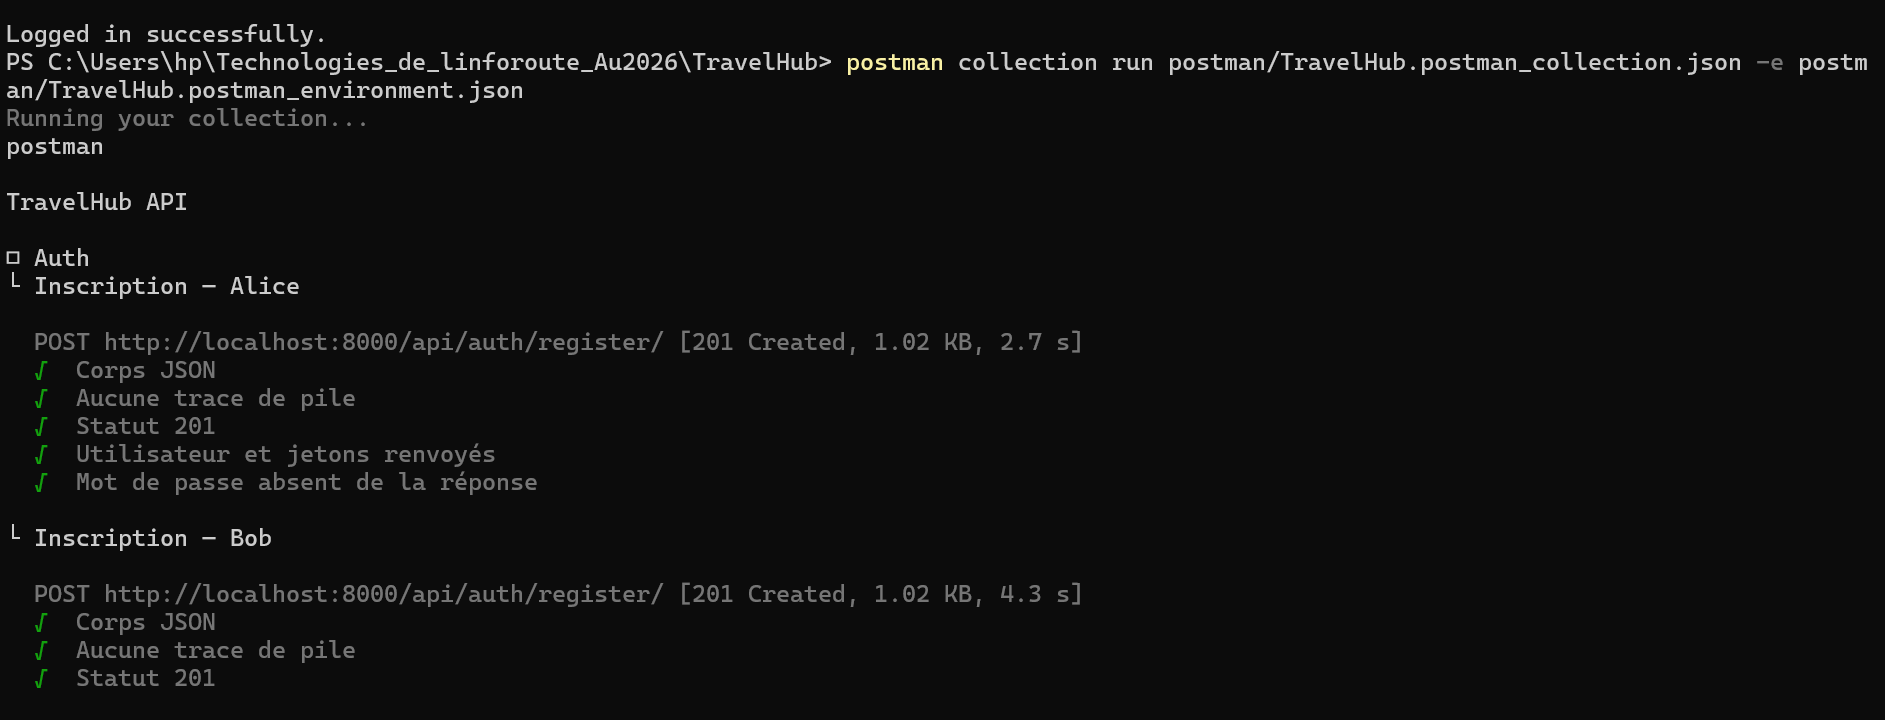
\includegraphics[width=\dimexpr\linewidth-2\fboxrule-2\fboxsep\relax]{figures/postman-runner.png}}%
  }{%
    \fbox{\parbox[c][3cm][c]{0.9\linewidth}{\centering\small
      Capture à insérer :\\[2pt] \texttt{figures/postman-runner.png}}}%
  }\\[6pt]
  \IfFileExists{figures/postman-runner1.png}{%
    \fbox{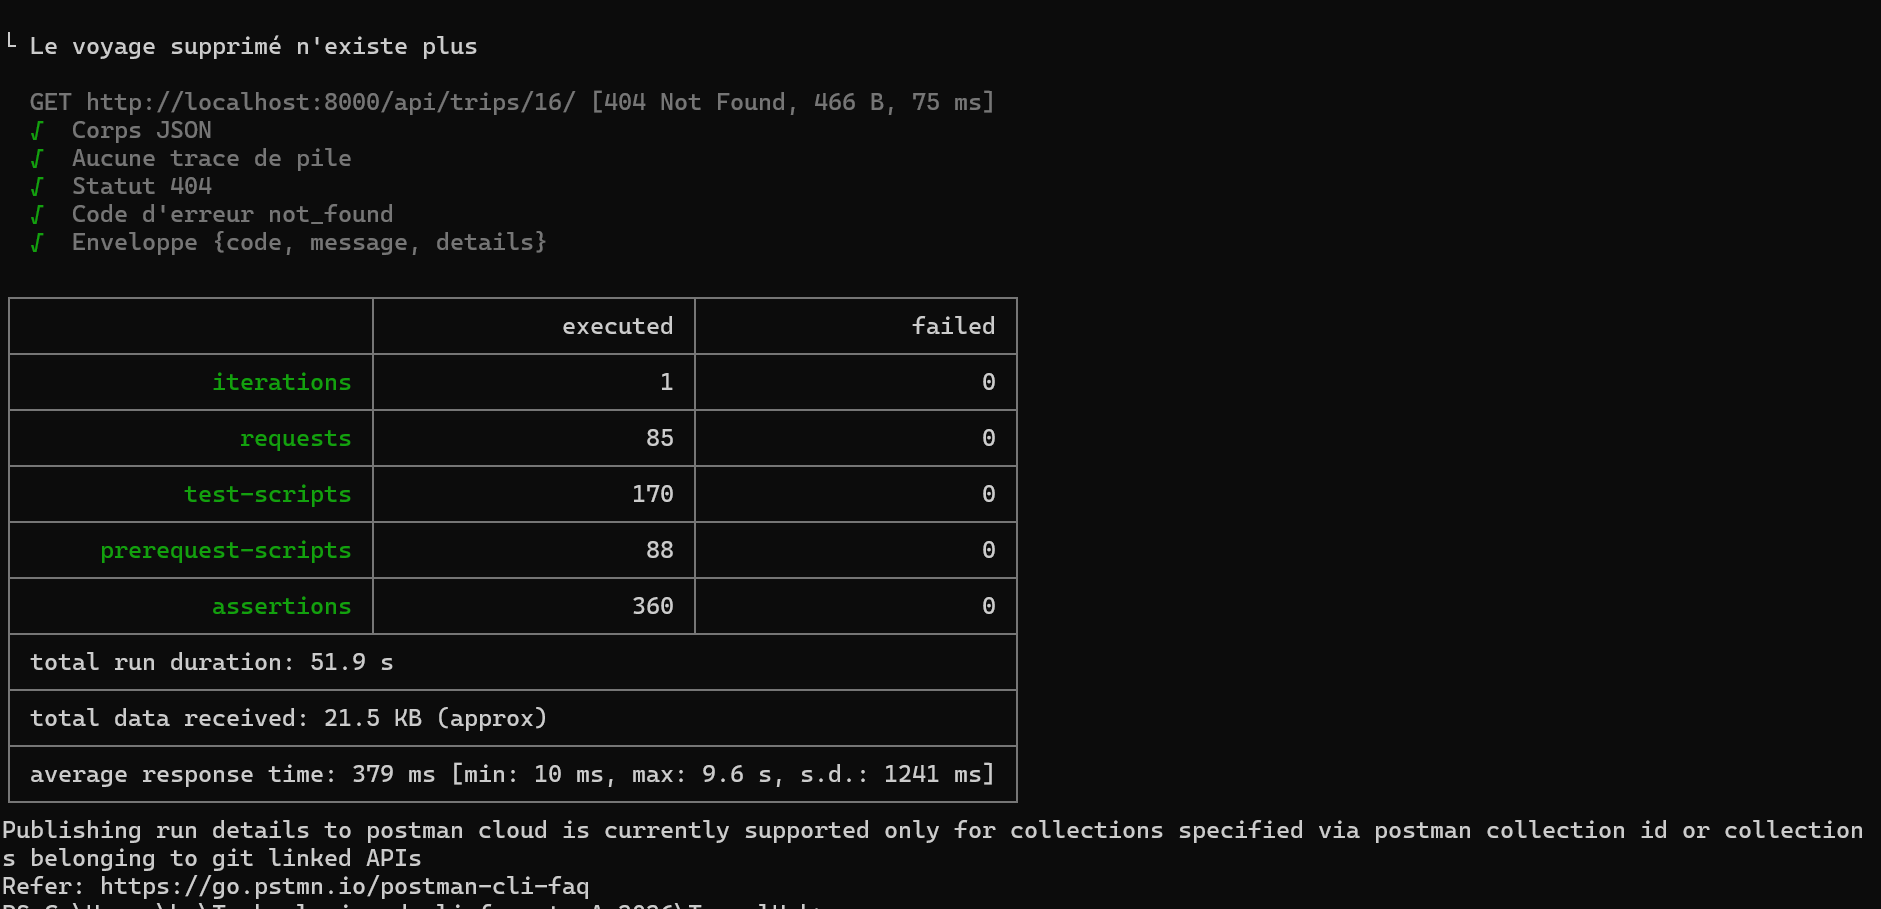
\includegraphics[width=\dimexpr\linewidth-2\fboxrule-2\fboxsep\relax]{figures/postman-runner1.png}}%
  }{%
    \fbox{\parbox[c][3cm][c]{0.9\linewidth}{\centering\small
      Capture à insérer :\\[2pt] \texttt{figures/postman-runner1.png}}}%
  }
  \caption{Exécution de la collection avec Postman CLI. En haut, le début de l'exécution avec les premières assertions. En bas, la dernière requête et le résumé (85 requêtes, 360 assertions, 0 échec).}
  \label{fig:postman}
\end{figure}

Les deux outils se complètent bien. Avec pytest, nous simulons les pannes qu'on ne peut pas provoquer quand on veut, comme un service externe en 500, un délai dépassé ou une panne au milieu d'une transaction. Postman, lui, vérifie le comportement de bout en bout, avec le vrai serveur et les vrais services externes.

\subsection{Qualité du code}

Ruff s'occupe de l'analyse statique (\code{ruff check}) et du formatage (\code{ruff format}). L'intégration continue lance ces deux vérifications avant les tests.
